\subsection{Systematic Investments Overview}

A schematic of a live 'production' trading strategy is shown below, but does not include everything else necessary to create the strategy (i.e., research tools).
\begin{figure}[H]
\centering
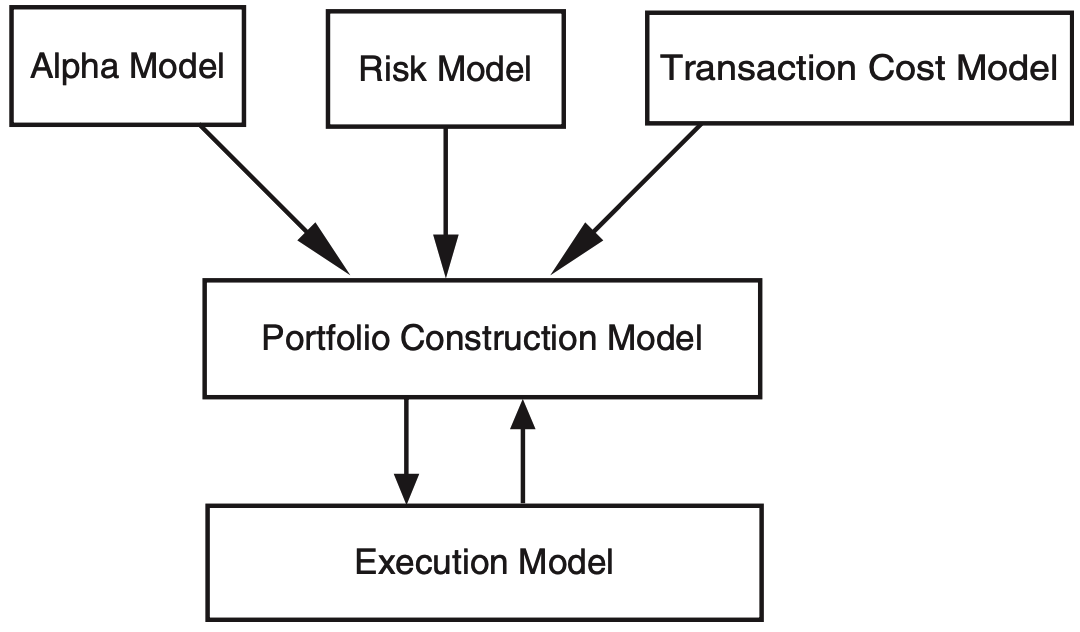
\includegraphics[scale=0.4]{intro/strategystructure}
\caption{Live 'production' trading strategy}
\end{figure}
The trading system has three modules:
\begin{enumerate}[label=\roman*.]
\setlength{\itemsep}{0pt}
\item Alpha model: predicts the future of the instruments considered for trading, i.e. directional alpha
\item Risk model: limits amount of exposure to factors that are unlikely to generate returns but could drive losses, i.e. directional exposure limit on an asset class
\item Transaction cost model: determine if the cost of the trades needed to migrate from current portfolio to new portfolio is desirable to the portfolio construction model.
\end{enumerate}
These models feed into a portfolio construction model that balances the tradeoffs of profit and risk to determine the best portfolio to hold. The model finds the differences in trades that need to be executed.\\
The execution model then takes the required trades, and using inputs such as urgency in which the trades need to be executed and dynamics of liquidity in the markets, executes the trades in an efficient and low cost manner.\\

\begin{method} \hlt{Chains of Production for Alpha Signals}
\begin{enumerate}[label=\roman*.]
\setlength{\itemsep}{0pt}
\item Data Curation: for collecting, cleaning, indexing, storing, adjusting, and delivering all data to production chain. Requires experts in market microstructure and data protocols such as FIX.
\item Feature Analysis: transform raw data into informative signals. Requires experts in information theory, signal extraction and processing, visualisation, labelling, weighting, classifiers, feature importance techniques. Feature analysts collect and catalogue libraries of findings.
\item Strategists: informative features are transformed into actual investment algorithms. Strategists will parse libraries of features for ideas to develop an investment strategy. Require data scientists with deep knowledge of financial markets and economy. Features may be discovered by black box, but strategy is developed in a white box.
\item Back-testers: assess profitability of investment strategy under various scenarios. Requires data scientists with deep understanding of empirical and experimental techniques. Good back-tested incorporates in analysis meta-information on how strategy was created.
\item Deployment Team: integrate strategy code into production line. Requires algorithm specialists and mathematical programmers. To ensure deployed solution is logically identical to prototype, and to optimise implementation sufficiently such that production latency is minimised.
\item Portfolio Oversight: once strategy is deployed, follows lifecycle.
\begin{enumerate}[label=\arabic*.]
\setlength{\itemsep}{0pt}
\item Embargo: initially, strategy is run on data observed after end date of backtest. If embargoed performance is consistent with backtest, strategy is promoted to next stage.
\item Paper Trading: strategy run on live, real-time feed. Performance accounts for data parsing latencies, calculation latencies, execution delays, and other time lapses between observation and positioning. 
\item Graduation: strategy manages real position, whether in isolation of as part of ensemble. Performance evaluated precisely, including attributed risk, returns, and costs.
\item Re-allocation: based on production performance, allocation is re-assessed frequently and automatically. Strategy allocation follows a concave function, Initial allocation is small. As time passes and strategy performs as expected, allocation is increased. Over time, performance decays and allocations become gradually smaller.
\item Decommission: if strategy perform below expectations for sufficiently extended period of time, strategy is discontinued.
\end{enumerate}
\end{enumerate}
\end{method}

\subsubsection{Alpha models}

Theory-driven models tests theories of why markets behave in a manner, and see if they can be used to predict the future. Strategies utilising price-related data are trend and mean reversion; strategies utilising fundamental data are value/yield, growth and quality. Usually more than one model is used in combination.

\begin{definition} \hlt{Theory Driven Models}
\begin{enumerate}[label=\roman*.]
\setlength{\itemsep}{0pt}
\item Trend Following: markets move in given direction long enough that the trend can be identified. As more data support the bull/bear thesis in an uncertain market, more market participants will adopt the same thesis and hence move the asset price to a new equilibrium.\\
Moving average crossover indicator strategy has less than one point of return for every point of downside risk taken, as market behaviour are unstable and episodic.
\item Mean Reversion: markets move in opposite direction to the prevailing trend. Short-term imbalances between buyers and sellers due to liquidity forces prices to move abruptly in one direction, which increases probability of trend reversion as liquidity issue is resolved.\\
Statistical arbitrage bets on convergence of prices of similar stocks whose prices have diverged.\\
Longer-term trends can occur despite smaller oscillations around these trends occurring in the shorter term, hence both strategies may be used in conjunction.
\item Value/Yield:  value strategies uses ratios of fundamental factor against the price of the instrument, inverted to keep the ratio consistent. The higher the yield, the cheaper the instrument.\\
Buying undervalued security and selling overvalued security is a \hlt{carry trade}. The difference between yield received and yield paid is the \hlt{carry}.\\
\hlt{Quant Long Short (QLS)} ranks stocks by attractiveness based on various factors such as value, then buy the higher-ranked stocks while shorting the lower-ranked stocks.
\item Growth: make predictions based on asset's expected or historically observed level of economic growth. Forward-looking growth expectations are typically used as a metric.\\
Growth is trending, and strongest growers are becoming more dominant relative to competitors. Macro growth factors may be used on foreign exchange, while micro growth factors may be used on companies.
\item Quality: All else being equal, it is better to long high quality and short low quality. Capital safety is important. Factors include earnings quality, equity-to-debt ratios etc.
\end{enumerate}
\end{definition}

Data-driven models are more difficult to understand, with more complicated mathematics. Relies on data mining, more technically challenging and far less widely practiced. Typically more used in high-frequency space, as they can discern how market behaves without caring about the economic theory or rational.

\begin{method} \hlt{Strategy Parameters}\\
An implementation approach requires a forecast target, time horizon, bet structure, investment universe, model specification, and run frequency.
\begin{enumerate}[label=\roman*.]
\setlength{\itemsep}{0pt}
\item Forecast Target: models may forecast direction, magnitude, duration of move, and may include probability into the forecast. Signal strength is of importance, defined by a larger expected return and/or higher likelihood of return. A higher level of signal strength results in a bigger bet taken on the position.
\item Time Horizon: models may have forecast horizons ranging from microseconds to years. There are more variability between short-term and long-term strategies, as short-term strategies are making very large number of trades compared to long-term strategies.
\item Bet Structure: models can be made to forecast an instrument relative in itself or to others. For relative forecasts, smaller clusters (pairs) or larger clusters (sectors) may be used. For pairs, few assets can be compared precisely and directly. Large cluster grouping may eliminate impact of general movement of the sector and hence focus on the relative movement of stocks within the sector, allowing for clearer distinction between group behaviour and idiosyncratic behaviour. Clusters may be created either via statistical methods or using heuristics (i.e., fundamentally defined industry groups).\\
Statistical methods may be fooled by data, leading to bad grouping. Heuristic grouping may be imprecise for conglomerates, and may be too rigid. Relative alpha strategies tend to exhibit smoother returns during normal times than intrinsic alpha strategies, but may face incorrect groupings during stressful periods. This may be mitigated by utilising several grouping techniques in concert.
\item Investment Universe: choices made on geography, asset class, instrument class, and exclusions. Liquidity is preferred so estimations of transaction costs are reliable. Large quantities of high quality data is required, which is found in highly liquid and developed markets. Instruments with consistent behaviour is preferred, hence biotech stocks are excluded due to sudden, violent price changes. Hence, the most common asset classes and instruments modelled are common stocks, futures (on bonds and equity indices) and forex.
\item Model Specification: focuses on definition of the strategy mathematically, and may be the source of alpha. Specification details in terms of machine learning or data mining techniques are also defined, to assist in fitting models to the data and setting parameter values. Refitting frequency is also defined to refresh the model and make it adapt to current market conditions; may lead to greater risk of overfitting.
\item Run Frequency: defined from monthly to real time frequency. Increasing frequency of runs lead to greater number of transactions and hence higher transaction costs, and risk of moving portfolio based on noisy data. Less frequency of runs lead to smaller number of larger-sized trades, hence may move the market with block trades; may also miss opportunities to trade at more favourable prices.
\end{enumerate}
\end{method}

\begin{method} \hlt{Blending of Models}\\
Most common approaches are linear models, nonlinear models, and machine learning models. If models are not combined, then several portfolios are constructed based on output from each model, then combined using portfolio construction techniques. The best method depends on the model.
\begin{enumerate}[label=\roman*.]
\setlength{\itemsep}{0pt}
\item Linear Models: require independence of factors, and each factor to be additive. To determine the weight of each alpha factor, multiple regression techniques may be used.
\item Nonlinear Models: used when factors are not independent, or the relationship changes over time. Conditional models base the weight of one factor on the reading of another factor. Rotational models assign weights of factors that fluctuate over time based on updated calculations of the various signal's weights, giving higher weights to factors with better performance recently.
\item Machine Learning Models: developing machine learning strategies takes as much effort to produce one true investment strategy as to produce a hundred. The complexities include data curation and processing, HPC infrastructure, software development, feature analysis, execution simulations, backtesting etc.\\
Decades ago, macroscopic alpha based on simple tools like econometrics are common, but this is quickly diminishing. Microscopic alpha however, becomes more abundant, but requires heavy ML tools.
\end{enumerate}
\end{method}


\subsubsection{Risk Models}

Risk models are indispensable tools in algorithmic trading, providing a quantitative framework to assess, monitor, and manage the inherent risks of financial markets. They not only serve to measure exposure but also guide portfolio construction, hedging strategies, and overall risk control.

\begin{method} \hlt{Factor-Based Models}\\
Factor-based models decompose asset returns into contributions from systematic factors and idiosyncratic components. The most common factors include:
\begin{enumerate}[label=\roman*.]
	\setlength{\itemsep}{0pt}
    \item \textbf{Market Factor:} Captures the overall movement of the market.
    \item \textbf{Size Factor:} Reflects the differential risk associated with companies of varying market capitalizations.
    \item \textbf{Value Factor:} Accounts for risk due to discrepancies between market prices and fundamental valuations.
    \item \textbf{Momentum Factor:} Measures the tendency of asset prices to continue in their current trajectory.
\end{enumerate}
This allows traders to understand which elements drive portfolio risk and adjust exposures accordingly.
\end{method}

\begin{method} \hlt{Statistical Models}\\
Statistical risk models leverage historical data and probabilistic techniques to quantify risk parameters.
\begin{enumerate}[label=\roman*.]
	\setlength{\itemsep}{0pt}
    \item \textbf{Historical Simulation:} Directly computing risk metrics from past return distributions.
    \item \textbf{Monte Carlo Simulation:} Generating a large number of potential future return scenarios to estimate risk under diverse conditions.
    \item \textbf{Parametric Methods:} Employing analytical formulas based on assumed return distributions to calculate key risk measures.
\end{enumerate}
These are useful for dynamically updating risk assessments as new market data become available.
\end{method}

\begin{method} \hlt{Limiting Size of Risk}\\
Quantitative risk models are designed to limit the size of exposures to enhance return consistency.
\begin{enumerate}[label=\roman*.]
	\setlength{\itemsep}{0pt}
    \item \textbf{Constraint Mechanisms:}
        \begin{enumerate}[label=\alph*.]
            \item \textbf{Hard Constraints:} Absolute limits imposed on position sizes, which may be set arbitrarily.
            \item \textbf{Penalty Functions:} Flexible constraints where positions can exceed the limit if the alpha model forecasts significantly higher returns, with penalties applied for surpassing the prescribed levels.
        \end{enumerate}
    \item \textbf{Risk Measurement Approaches:}
        \begin{enumerate}[label=\alph*.]
            \item \textbf{Longitudinal Analysis:} Evaluates risk by assessing the volatility of an instrument over time.
            \item \textbf{Dispersion Analysis:} Measures risk by analyzing the correlation or covariance between assets.
        \end{enumerate}
\end{enumerate}
These methods can be applied to single positions, groups of positions (such as sectors or asset classes), different types of risk exposures, and overall portfolio leverage.
\end{method}

\begin{method} \hlt{Limiting the Types of Risk}\\
To eliminate unintentional exposure as there is no expectation of being compensated sufficiently for accepting them. This can be achieved the following measures:
\begin{enumerate}[label=\roman*.]
	\setlength{\itemsep}{0pt}
    \item \textbf{Market Exposure Restriction:} Focus on specific market segments to avoid undue exposure to volatile or unpredictable markets.
    \item \textbf{Leverage Management:} Limit the use of leverage by enforcing conservative leverage ratios to mitigate amplified losses.
    \item \textbf{Stop-Loss Policies:} Implement strict stop-loss rules to automatically exit positions that breach predetermined loss thresholds.
    \item \textbf{Position Size Controls:} Cap individual position sizes relative to overall portfolio risk, ensuring no single trade unduly influences portfolio performance.
    \item \textbf{Regular Risk Assessments:} Continuously monitor risk metrics and adjust risk parameters to reflect evolving market conditions.
\end{enumerate}
\end{method}


\subsubsection{Transaction Cost Models}

A trade is executed only if it improves the probability or magnitude of a return (as predicted by alpha model) or reduces likelihood or extent of a loss (as determined by risk model). However, this improvement must be greater than cost of trading. Note that transaction cost model is intended not to minimize trading costs directly, but rather to inform the portfolio construction engine of the costs associated with executing a given trade.

\begin{remark} \hlt{Transaction Cost Components}
\begin{enumerate}[label=\roman*.]
\setlength{\itemsep}{0pt}
    \item \textbf{Commissions and Fees:} These are payments made to brokerages (for accessing other market participants), exchanges (for enhanced transaction security), and regulators (for maintaining operational infrastructure). In the context of quantitative trading, where bank infrastructure is utilized, brokerage commissions tend to be minimal on a per-trade basis.\\[1mm]
    Brokers also charge clearing and settlement fees. \emph{Clearing} involves activities such as regulatory reporting and monitoring, tax handling, and failure management, all of which occur before settlement. \emph{Settlement} is the final delivery of securities in exchange for full payment.
    \item \textbf{Slippage:} This refers to the change in price between the moment the trading system decides to execute a transaction and the time the order is actually sent to the exchange. Trend-following strategies tend to experience more slippage because the assets are already moving in the desired direction, whereas mean-reverting strategies are less affected. Reduced latency to market minimizes slippage, while higher asset volatility increases it.  
    \item \textbf{Market Impact:} This measures the extent to which an order influences the market through its demand for liquidity. The market impact remains uncertain until after the trade is executed. Additionally, there can be an interaction between slippage and market impact (i.e., selling during an upward trending market).
\end{enumerate}
\end{remark}

\begin{definition} \hlt{Types of Transaction Cost Models}
\begin{enumerate}[label=\roman*.]
\setlength{\itemsep}{0pt}
    \item \textbf{Flat Model:} Assumes that the cost of trading remains constant regardless of the order size. This model is appropriate when the traded size is nearly uniform and liquidity remains stable.
    \item \textbf{Linear Model:} In this model, the trading cost increases at a constant rate relative to the order size. It provides a better estimate than the flat model.  
    \item \textbf{Piece-Wise Linear Model:} This approach employs piece-wise linear functions to model costs. It strikes a balance between simplicity and accuracy, offering improved precision compared to flat or linear models.
    \item \textbf{Quadratic Model:} Although the most computationally intensive, the quadratic model delivers the highest accuracy in cost estimation.
\end{enumerate}
\end{definition}


\subsubsection{Portfolio Construction Models}

Comes in two major forms: rule-based, optimisers. Rule-based models are based on heuristics, can be exceedingly simple or rather complex, and derived from human experience (trial and error). Optimisers comprises of an objective function and uses algorithms to reach the end goal.

\begin{definition} \hlt{Rule-Based Models}
\begin{enumerate}[label=\roman*.]
\setlength{\itemsep}{0pt}
\item Equal Position Weighting: used if portfolio manager believes that if a position is good enough to own, no other information is needed in determining its size. Strength of signal is not used as input in weighting.\\
Model assumes that there is sufficient statistical strength and power to predict not only direction but also magnitude relative to other forecasts in the portfolio. Portfolio takes few large bets on 'best' forecast, many smaller bets on less dramatic forecasts; may take excess risk in an idiosyncratic event on a seemingly attractive position, resulting in adverse selection bias.
\item Equal Risk Weighting: adjust position sizes inversely to volatilities or a measure of risk. More volatile positions given smaller allocations, less volatile positions given larger allocations.\\
When unit of risk is equalised, it is almost always a backward-looking measurement such as volatility. If volatility changes with time, then model will be misled.
\item Alpha-Driven Weighting: position size based primarily on alpha model. Alpha signal determines size of position, but usually with size limits. Constraints used also includes limits on size of total bet on a group. May also have a function that relates the magnitude of forecast to size of position.\\
If model used in futures trend following, might suffer sharp drawdowns. Reliance on accuracy of alpha.
\item Decision-Tree Weighting: decision path to arrive at the allocation for given instrument, depending on type of alpha model and type of instrument. Constraints may include percentage limits for allocation.\\
Model size grows dramatically if more alpha models or mode types of positions are included.
\end{enumerate}
\end{definition}

\begin{remark} \hlt{Optimisers Models Parameters}\\
Harry Markowitz's mean variance optimisation (MVO) as the pioneer model. Models are based on principles of modern portfolio theory (MPT). Inputs include asset expected return (mean), asset variance, expected correlation matrix. Other inputs include size of portfolio in currency terms, desired risk level (volatility or expected drawdown), and other constraints such as liquidity, universe limits.\\
Model uses an objective function and an algorithm to seek the goal, usually maximising return of portfolio relative to volatility of portfolio returns.
\begin{enumerate}[label=\roman*.]
\setlength{\itemsep}{0pt}
\item Expected Return: alpha models as basis of expected return, which also includes expected direction.
\item Expected Volatility: stochastic volatility forecasting methods is commonly used, as volatility may have high and low periods, with occasional jumps. GARCH model is most used.
\item Expected Correlation: as instrument correlations are not stable over time, it is more appropriate to group assets together before computing correlation within the group.
\end{enumerate}
\end{remark}

\begin{method} \hlt{Optimisation Techniques}
\begin{enumerate}[label=\roman*.]
\setlength{\itemsep}{0pt}
\item Unconstrained Optimisation: most basic form with no constraints. Might provide a single-instrument portfolio, where all money will be invested in instrument with highest risk-adjusted return.
\item Constrained optimisation: constraints include position limits, limits on various groupings of instruments. Might result in constraints driving the portfolio construction more than the optimiser.
\item Black-Litterman Optimisation: blends investor expectations with a degree of confidence about those expectations, and these with historical precedent evident in the data. Adjusts historically observed correlation levels by utilising investor's forecast of return for the various instruments.
\item Grinold and Kahn's Approach: builds a portfolio of signals, instead of sizing positions. To build factor portfolios, each of which are usually rule-based portfolios based on a single type of alpha forecast. Each portfolio backtested, then series of returns are then treated as instruments of a portfolio by the optimiser.\\
Number of factor portfolios is more manageable, usually not more than 20. What is optimised is then a handful of factor portfolios. The model allows for inclusion of risk model, transaction cost model, portfolio size, and risk targets as inputs.
\item Resampled Efficiency: to improve the inputs to optimisation by addressing oversensitivity to estimation error. To resample data using Monte Carlo simulation to reduce estimation error in inputs to the optimiser.
\item Data-Mining Approaches: machine learning techniques such as supervised learning or genetic algorithms used, as MVO involves searching many possible portfolios to find the best.
\end{enumerate}
\end{method}

\subsubsection{Execution Model}

Two basic ways to execute trade: through electronic, or through human intermediary. For electronic execution, achieved through direct market access (DMA), which allows traders to utilise the infrastructure and exchange connectivity of brokerage firms to trade directly on electronic markets.\\
Execution algorithms can be acquired through building, using broker's, or a third-party software vendors.\\
Brokerages offer portfolio bidding, where the 'blind' portfolio for transaction is described by characteristics such as valuation ratios of longs and shorts, sector breakdown, market capitalisation etc. Broker then quote a fee in basis points in terms of the gross market value of portfolio traded. Hence, certainty is provided by the broker to the trader. Once agreement reached, broker receives fee and assumes risk of trading out the portfolio at future market prices, which may be better or worse than prices guaranteed.

\begin{remark} \hlt{Order Execution Algorithm Parameters}
\begin{enumerate}[label=\roman*.]
\setlength{\itemsep}{0pt}
\item Aggressive vs Passive: algorithm make decision of passive vs aggressive order, depending on how immediately the trader wants to do the trade. Market orders are considered aggressive. Limit order at current best order is fairly aggressive, while limit order below current bid is passive.\\
Many exchanges pay providers of liquidity for placing passive orders, charging traders for using liquidity provided. Orders that cross the spread are using liquidity by using a passive order placed by another trader, reducing liquidity available. Paying for liquidity sweetens deal for passive order, only if order is actually executed; passive trader gets better transaction price and a commission rebate from the exchange.\\
Momentum strategies uses more aggressive orders; mean reversion uses more passive orders. A stronger, more certain signal will be executed with greater aggressiveness than a weaker or less certain signal. A middle ground will be to put limit orders between best current bid and offer.
\item Large vs Small Order: a large order may be broken into many smaller orders over a window of time, but risk price moving in adverse direction. Size of chunk depends on transaction cost model estimate, and analysis of correct level of aggressiveness.
\item Hidden vs Visible Order: a queue as a visible order gives away a bit of information. Hidden order will provide no information to the market, staving off imbalances, but reduces priority of trade in the queue.\\
Algorithmic trading utilising hidden order is 'iceberging', which is taking a single larger order and chopping it into many smaller chunks, most posted to order book as hidden orders.
\item Order Routing: if there are several pools of liquidity for the same instrument, smart order routing will be used, which determines which pool of liquidity is most suitable for sending a given order. Depth of liquidity on various ECNs and connectivity speeds are also considered in smart order routing.
\item Cancelling and Replacing Orders: traders may place larger number of orders with no intention of execution, then rapidly cancelling them and replacing them with other orders. This allows gaining of information on how market responds to the changing depth of the book, providing information on how to profit from the pattern of reaction. If trader wants to buy a large number of shares, he may enter a large number of small orders to sell the shares further away from market and cancel, improving market perception.
\end{enumerate}
\end{remark}

\begin{definition} \hlt{High Frequency Trading}\\
Alpha driving strategies on extremely near-term bets (seconds or less) are \hlt{microstructure alphas}, focusing on liquidity patterns in order book. Larger quants may also use this to guide execution models, improving costs of entering trades. Small differences over a single trade add up significantly in the long run.To trade microstructure alpha as independent high frequency strategies, large investments in infrastructure and research must be done.\\
Machine learning techniques may also be used to discern patterns in execution of other player orders. The more inferior the execution models, the easier it is to discern the pattern, allowing the ML strategy to profit from these patterns in the future. Patterns in the shorter timescale are somewhat stable.
\end{definition}

\begin{definition} \hlt{HFT Shark Strategy}\\
Designed to detect large orders that are iceberged, by sending series of very small trades; if each of these small orders get filled quickly, this may be a sign of a large and iceberged order. The shark simply front-run this large, hidden order by placing visible trades in front of the iceberged order. The iceberg strategy must then push prices up to execute trades. When the iceberged order is complete, prices will be pushed up favourably for the shark, which can then exit the position with a quick and relatively riskless profit.
\end{definition}

\begin{remark} \hlt{HFT Trading Infrastructure}\\
Using a broker that act as trading agent allows the infrastructure requirements to be handled by the broker, instead of dealing with the regulatory and other constraints. \\
High frequency strategies may use colocation or sponsored access. Colocation setup is where trader attempts to place trading servers as physically close to the exchange as possible.\\
Financial Information eXchange (FIX) protocol is the choice of real-time electronic communication among users. The software that implements the FIX protocol is free and open source (FIX engine). High frequency traders will likely build their own FIX engines to ensure optimal speeds.
\end{remark}



\subsubsection{Research}

\begin{definition} \hlt{Scientific Method}
\begin{enumerate}[label=\arabic*.]
\setlength{\itemsep}{0pt}
\item Researcher observe a phenomenon in the market and construct a theory.
\item Researcher seeks out information to test the theory.
\item Researcher tests the theory, and with enough confidence, risk some capital on the validity of the theory.
\end{enumerate}
\end{definition}

\begin{remark} \hlt{Sources of Alpha Idea Generation}
\begin{enumerate}[label=\arabic*.]
\setlength{\itemsep}{0pt}
\item Observing the market, using the scientific method to test the theory
\item Academic literature, requiring significant time to read academic journals, working papers, and conference presentations for ideas. Literature from other fields such as astronomy, physics, or psychology, may provide ideas relevant to quant finance problems.
\item Migration of a researcher or portfolio manager from one quant shop to another.
\item Lessons from activities of discretionary traders
\end{enumerate}
\end{remark}

\begin{remark} \hlt{Model Quality Assessment}
\begin{enumerate}[label=\roman*.]
\setlength{\itemsep}{0pt}
\item \textbf{Cumulative Profit Graph:} A smooth profit curve is ideal; if the graph shows long periods of inactivity or exhibits sharp, erratic losses and gains, it may signal issues with the model.
\item \textbf{Average Annual Rate of Return:} Indicates the historical performance level of the strategy.
\item \textbf{Variability of Returns:} Lower variability in returns is preferable, as it suggests consistency. Examining the "lumpiness"—the share of total returns derived from periods significantly above average—can further measure return consistency.
\item \textbf{Peak-to-Valley Drawdowns:} Measures maximum decline from any cumulative peak in the profit curve. Lower drawdowns, along with shorter recovery periods after drawdowns, reflect a more robust strategy.
\item \textbf{Predictive Power:} The R-squared statistic can be employed to assess how much of the variability in the predicted asset is explained by the model. For example, an exceptionally high \( R^2 \) (around 0.05 out of sample) may warrant further scrutiny. Additionally, bucketing instrument returns by deciles can help verify whether the model categorizes them accurately.
\item \textbf{Percentage of Winning Trades and Winning Time Periods:} Determines whether the strategy relies on a small number of highly profitable trades or on a larger volume of moderately successful trades.
\item \textbf{Risk-Adjusted Return Ratios:} Evaluate statistics such as the Sharpe ratio, information ratio, Sterling ratio, Calmar ratio, and Omega ratio to assess the balance between returns and risk.
\item \textbf{Relationship with Other Strategies:} Consider the incremental value provided by a new strategy by comparing its performance with existing strategies, both independently and in combination.
\item \textbf{Time Decay:} Examine how the returns of the strategy are affected if trades are initiated on a lagged basis after receiving a trading signal. This helps to determine the sensitivity of the strategy to the timeliness of information and the degree of market saturation.
\item \textbf{Sensitivity to Specific Parameters:} A high-quality strategy should show only minor variations in outcomes with small changes in its parameters; large fluctuations may indicate overfitting.
\item \textbf{Overfitting:} By plotting parameter values against the corresponding outcomes, one should observe a relatively flat curve with no abrupt jumps. Models that are parsimonious—that is, those that rely on fewer parameters—tend to be less prone to overfitting.
\end{enumerate}
\end{remark}

\begin{remark} \hlt{Other Considerations in Model Testing}\\
It is crucial to note that overestimating trading costs can lead to holding positions longer than optimal, whereas underestimating these costs might result in excessive portfolio turnover and a detrimental bleed from trading expenses. Moreover, assumptions regarding the availability of short positions must be carefully considered, especially with respect to hard-to-borrow lists.
\end{remark}


\subsubsection{Risk Assessment}

\begin{definition} \hlt{Model Risks}\\
Quant models has model risk, the risk that the model does not accurately describe, match, or predict the real-world phenomenon. Each component of the quant model may all have model risk.
\begin{enumerate}[label=\roman*.]
\setlength{\itemsep}{0pt}
\item Inapplicability of Modelling: occurs when quant model is mistakenly applied to a problem. May also occur with misapplication of a technique to a given problem.
\item Model Misspecification: occurs when the model doesn't fit the real world. Model may work fine most of the time, but fail when an extreme event occurs.
\item Implementation Errors: erors in programming or architecting systems. Architectural error may also occur when models are loaded in a wrong sequence.
\end{enumerate}
\end{definition}

\begin{definition} \hlt{Regime Change Risk}\\
Quant models are based on relationships prevalent in historical data. If there is a regime change, the historical relationships and behaviour may be altered, hence the model may lose effectiveness.
\end{definition}

\begin{definition} \hlt{Exogenous Shock Risk}\\	
Risks driven by information that is not internal to the market, i.e., terrorist attacks, start of wars, bank bailouts, change in regulation such as in shorting rules. May require discretionary overrides.
\end{definition}

\begin{definition} \hlt{Contagion Risk}\\
Happens when other investors hold the same strategies. First part of risk factor relates to how crowded the quant strategy is. Second part relates to what else is held by other investors that could force them to exit the quant strategy in a panic (ATM effect).\\
Quant liquidation criss may be driven by size and popularity of quantitative strategies, subpar returns from operators leading up to the crisis, the practice of funds cross-collateralising many strategies against each other, and risk targeting (risk managers target a specific level of volatility for their funds or strategies).
\end{definition}

\begin{method} \hlt{Risk Monitoring Methods}
\begin{enumerate}[label=\roman*.]
\setlength{\itemsep}{0pt}
\item Exposure Monitoring Tools: with current positions held, the positions are grouped for the various exposures (i.e., valuation, momentum level, volatility) to monitor gross and net exposure to various sectors and industries, buckets of market capitalisation, various style factors.
\item Profit and Loss Monitors: with current portfolio, compare that with previous day closing price. Intraday performance charts are used. May also look at source of profit, hit rate (percentage of time strategy makes money on a given position).
\item Execution Monitors: shows progress of executions, i.e., which orders are currently being worked on, which ones are completed, with transaction size and prices. Fill rates for limit orders are used for more passive execution strategies. Slippage and market impact are also monitored.
\item System Performance Monitors: checks for software and infrastructure errors. Checks performance of CPUs, speeds of various stages of automated processes, latency in communication of messages.
\end{enumerate}
\end{method}
